%%%%%%%% EEML 2026 Extended Abstract — v4 %%%%%%%%%%
\documentclass{article}
\usepackage{microtype}
\usepackage{graphicx}
\usepackage{subfigure}
\usepackage{booktabs}
\usepackage{hyperref}
\newcommand{\theHalgorithm}{\arabic{algorithm}}
\usepackage[accepted]{icml2025}
\usepackage[
  letterpaper,
  left=0.75in,
  right=0.75in,
  top=1.0in,
  bottom=1.0in,
  headheight=10pt,
  headsep=10pt
]{geometry}
\usepackage{amsmath}
\usepackage{amssymb}
\usepackage{mathtools}
\usepackage[capitalize,noabbrev]{cleveref}

\begin{document}

\twocolumn[
\icmltitle{Graph Construction from a Statistical Vocabulary}

\icmlsetsymbol{equal}{*}

\begin{icmlauthorlist}
\icmlauthor{Will Edibam}{usyd,dns}
\icmlauthor{Ben Fulcher}{usyd,dns}
\end{icmlauthorlist}

\icmlaffiliation{usyd}{The University of Sydney, Australia}
\icmlaffiliation{dns}{Dynamics and Neural Systems Group}

\vskip 0.3in
]

\begin{abstract}
This extended abstract presents work in preparation that applies our group's \texttt{pyspi} framework \citep{cliff2023} to the problem of graph construction for graph neural networks on multivariate time series. Graph construction is the critical upstream design variable in these pipelines, yet existing methods either commit to a single pairwise statistic or learn edges from latent embeddings with no statistical semantics. We parameterise construction over a vocabulary of $K {\approx} 125$ named pairwise statistics --- causal, spectral, linear, information-theoretic --- and jointly learn which are task-relevant. On synthetic topology classification, vocabulary-based models achieve $100\%$ macro F1 where symmetric baselines plateau at $59\%$ and latent baselines remain at chance. The learned weight vector recovers spectral Granger causality as the dominant coupling mode --- an interpretable statistical signature that latent methods structurally cannot produce.
\end{abstract}

%-----------------------------------------------------------------------
\section{Introduction}
\label{sec:intro}
%-----------------------------------------------------------------------

Message-passing neural networks (MPNNs) propagate information along relational structure \citep{gilmer2017,battaglia2018}. For multivariate time series (MTS), this structure is unobserved and must be constructed from data. The construction choice is the critical design variable: \citet{qi2025} showed that message-passing \emph{consistently degrades} when graph construction is naive, and \citet{liu2025} found substantial variation across 239 pairwise statistics benchmarked on the same neuroimaging data. Yet in every existing GNN pipeline, this choice is made once by the practitioner, before learning begins.

Current practice follows two regimes, both with fundamental limitations. Fixing the graph from a single statistic --- Pearson correlation \citep{bullmore2009}, transfer entropy \citep{duan2023} --- commits to one notion of dependence; if the task-relevant coupling is directed, nonlinear, or frequency-specific, the operator becomes the bottleneck. Learning the graph from latent embeddings \citep{kipf2018,wu2019,wu2020} recovers flexibility but sacrifices semantics: even NRI's discrete edge types \citep{kipf2018}, the most semantically structured latent approach, are learned categories with no pre-specified statistical meaning, and attention-based methods \citep{sriramulu2023} that initialise from statistics overwrite them during training. In scientific domains where the graph is the object of study --- neuroscience, climate, genomics --- this absence of statistical semantics is a fundamental limitation.

A concrete instance of why the choice matters: consider three VAR(1) motifs --- chain ($A {\to} B {\to} C$), fork ($A {\leftarrow} B {\to} C$), collider ($A {\to} B {\leftarrow} C$). Chain and fork are Markov-equivalent \citep{verma1990}: they share the same skeleton and v-structures, so any symmetric statistic assigns them identical edge weights regardless of sample size. No MPNN on such a graph can exceed $2/3$ accuracy on the three-class problem. Directed statistics --- where $f(X_i, X_j) \neq f(X_j, X_i)$ --- break this equivalence.

We propose a third regime: parameterise graph construction over a \emph{vocabulary} of $K$ named pairwise statistics computed via \texttt{pyspi} \citep{cliff2023}, spanning six complementary families: causal (transfer entropy, Granger causality, spectral GC --- \emph{asymmetric}), spectral (coherence, PLV), linear (covariance), information-theoretic (MI), distance (DTW), and rank (Spearman). A learned weight vector $\mathbf{w} \in \mathbb{R}^K$, jointly optimised with the MPNN, identifies which statistics are task-relevant. This follows \citet{velickovic2022}: rather than re-learning what ``connectivity'' means from raw data, we supply structured prior knowledge about pairwise dependence and let end-to-end learning select from it. The learned $\mathbf{w}$ is itself a scientific output: a named, testable hypothesis about which form of coupling drives the task.

%-----------------------------------------------------------------------
\section{Method}
\label{sec:method}
%-----------------------------------------------------------------------

Given $X \in \mathbb{R}^{M \times T}$, we compute $K$ statistics per ordered channel pair via \texttt{pyspi} \citep{cliff2023}, yielding a descriptor tensor $\mathbf{E} \in \mathbb{R}^{M \times M \times K}$. Graph construction is a linear probe of this descriptor space:
%
\begin{equation}
\label{eq:adj}
A_{ij} = \mathrm{softplus}\!\left(b + \mathbf{w}^\top \mathbf{E}_{ij}\right), \quad \text{top-}d \text{ per node}
\end{equation}
%
with $K {+} 1$ learnable parameters. The linearity is deliberate \citep[cf.][]{alain2017}: if the vocabulary is well-structured, a linear function suffices and $\mathbf{w}$ remains directly interpretable. Group lasso regularisation \citep{yuan2006} over the six SPI families encourages family-level selection:
%
\begin{equation}
\label{eq:loss}
\mathcal{L} = \mathcal{L}_{\mathrm{task}} + \lambda_1 \|\mathbf{w}\|_1 + \lambda_g \sum_{g \in \mathcal{G}} \|\mathbf{w}_g\|_2
\end{equation}

Retained edges carry the full descriptor $\mathbf{E}_{ij}$ as attributes. An edge network $\phi(\mathbf{E}_{ij}) {=} \mathrm{MLP}(\mathbf{E}_{ij})$ conditions messages on the statistical content of each edge:
%
\begin{footnotesize}
\begin{equation}
\mathbf{m}_{ij} {=} \mathrm{MLP}\!\left(\mathbf{h}_j \| \mathbf{h}_i \| \phi(\mathbf{E}_{ij})\right)\!, \;\; \mathbf{h}_i' {=} \mathbf{h}_i {+} \mathrm{LN}\!\left(\textstyle\sum_j A_{ij}\,\mathbf{m}_{ij}\right)
\end{equation}
\end{footnotesize}
%
The vocabulary thus plays a dual role: it determines \emph{which edges exist} (via $\mathbf{w}$) and \emph{what information flows along them} (via $\phi$). Global pooling produces graph-level predictions. Training: Adam, LR warmup (60 epochs), cosine decay, restart selection (best of 2 initialisations per seed).

% NOTE: small single-column pipeline schematic can go here if ready
% \begin{figure}[t]
% \includegraphics[width=\columnwidth]{figures/pipeline_schematic.pdf}
% \caption{Pipeline: MTS $\to$ pyspi $\to$ $\mathbf{E}$ $\to$ learned $\mathbf{w}$ $\to$ sparse directed graph $\to$ MPNN.}
% \end{figure}

%-----------------------------------------------------------------------
\section{Experiments}
\label{sec:experiments}
%-----------------------------------------------------------------------

\textbf{Setup.} $M{=}10$ node VAR(1) processes ($T{=}500$) with one of three directed motifs (chain, fork, collider) embedded among 7 nuisance AR(1) channels. Coupling $\alpha \sim U(0.3, 0.7)$; 1500 instances/class; $K{=}125$ after filtering; 30 random seeds. This is a controlled test of the theory: chain and fork produce \emph{identical} symmetric pairwise statistics.

% === FIGURE 1 ===
\begin{figure*}[t]
\vskip 0.1in
\begin{center}
\subfigure[Sample efficiency]{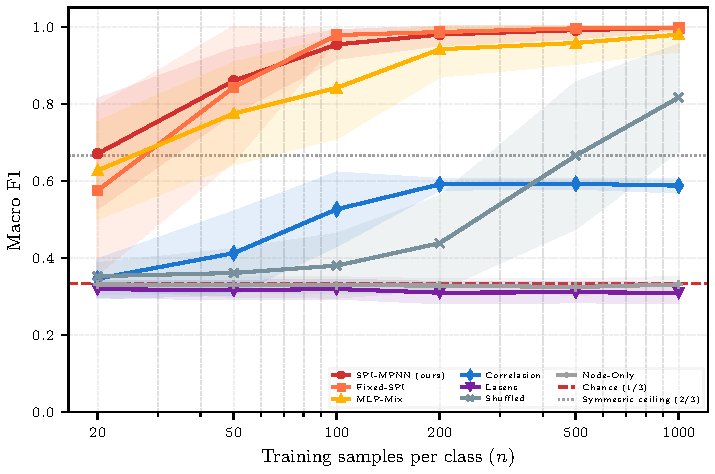
\includegraphics[width=0.62\textwidth]{figures/fig2a_sample_efficiency.pdf}\label{fig:efficiency}}
\hfill
\subfigure[Statistical signature]{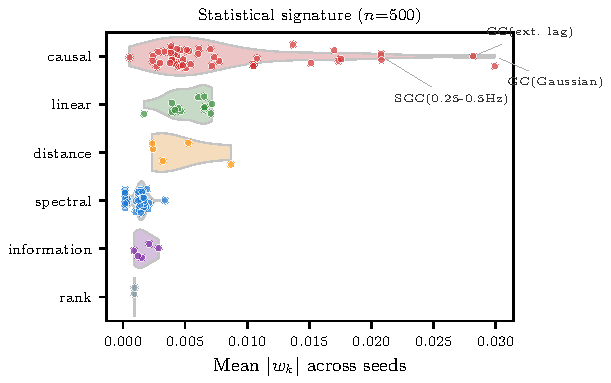
\includegraphics[width=0.35\textwidth]{figures/fig1c_family_violin.pdf}\label{fig:signature}}
\caption{(a)~Vocabulary-based models reach near-perfect F1 from $n{=}100$ while Correlation plateaus below the $2/3$ ceiling and Latent remains at chance. Red dashed: $1/3$ chance; grey dotted: $2/3$ symmetric ceiling. (b)~Family $L_2$ norms of learned $\mathbf{w}$ at $n{=}500$: the causal family dominates, with individual dot weights revealing spectral Granger causality as the top-weighted statistic.}
\label{fig:main}
\end{center}
\vskip -0.2in
\end{figure*}

\begin{table}[ht]
\caption{Macro F1 (\%, 30 seeds, $\pm$1 s.d.).}
\label{tab:main}
\vskip 0.05in
\begin{center}
\begin{small}
\begin{tabular}{lcccccc}
\toprule
$n$/cls & SPI & Fixed & E-Abl. & Corr. & Latent & Node \\
\midrule
20   & \textbf{67}{\scriptsize$\pm$14} & 58{\scriptsize$\pm$22} & 40{\scriptsize$\pm$15}  & 35{\scriptsize$\pm$5}  & 32{\scriptsize$\pm$2} & 33{\scriptsize$\pm$2}  \\
50   & \textbf{86}{\scriptsize$\pm$8}  & 84{\scriptsize$\pm$19} & 42{\scriptsize$\pm$16}  & 41{\scriptsize$\pm$11} & 32{\scriptsize$\pm$2} & 33{\scriptsize$\pm$2}  \\
100  & 95{\scriptsize$\pm$4}  & \textbf{98}{\scriptsize$\pm$1}  & 58{\scriptsize$\pm$26}  & 53{\scriptsize$\pm$9}  & 32{\scriptsize$\pm$2} & 33{\scriptsize$\pm$2}  \\
500  & 99{\scriptsize$\pm$2}  & \textbf{100}{\scriptsize$\pm$.3}& 93{\scriptsize$\pm$11}  & 59{\scriptsize$\pm$1}  & 31{\scriptsize$\pm$2} & 32{\scriptsize$\pm$2}  \\
1000 & \textbf{100}{\scriptsize$\pm$.4}& 100{\scriptsize$\pm$.3}& 96{\scriptsize$\pm$7}   & 59{\scriptsize$\pm$2}  & 31{\scriptsize$\pm$2} & 33{\scriptsize$\pm$2}  \\
\bottomrule
\end{tabular}
\end{small}
\end{center}
\vskip -0.15in
\end{table}

\textbf{The vocabulary is the contribution, not the architecture.} All SPI-consuming models dramatically outperform non-SPI baselines --- the gap is not marginal but the difference between near-perfect classification and chance. Fixed-SPI, which feeds the vocabulary as dense edge features on a fully connected graph with no learned topology, matches SPI-MPNN. This confirms that the \emph{representation of pairwise dependence} matters more than the mechanism used to construct edges from it. Critically, the oracle-best single statistic (spectral GC) achieves 87\% at $n{=}100$ but with catastrophic seed failures (std 22\%, vs SPI-MPNN's 4\%); at $n{=}20$ it falls to 36\%, below Correlation. The full vocabulary eliminates these failures entirely (std ${\leq}2\%$ at $n {\geq} 50$) through the diversity of 125 complementary estimators: many noisy views of pairwise dependence, when combined, are more stable than any single view --- however well-specified that view may be.

\textbf{Symmetric baselines confirm the theory.} Correlation never exceeds 59\%, well below the $2/3$ Markov-equivalence ceiling. The latent model \citep[cf.][]{wu2019} remains at chance (31--32\%) across all sample sizes --- node-level embeddings without statistical priors cannot access the chain--fork distinction. These are expressiveness limitations of symmetric graph construction, exactly as predicted.

\textbf{An interpretable statistical signature.} Under group lasso, the causal family (48 SPIs) carries ${\sim}3.5{\times}$ the $L_2$ norm of the next family (\cref{fig:main}b). The five highest-weighted individual SPIs are all spectral and time-domain Granger causality variants in the 0.25--0.5\,Hz band --- matching the generating process's causal structure \citep{geweke1982}. An edge-ablation study (same topology, zeroed edge features) drops F1 to 93$\pm$11\%, confirming the MPNN uses the statistical content of edges, not merely the topology (full ablation results in Appendix~\ref{app:ablation}).

This is the form of output that latent graph learners cannot produce: \emph{``the relational structure in this task is best captured by spectral Granger causality in the 0.25--0.5\,Hz band.''} On real-world MTS, the same mechanism would identify which notion of coupling --- coherence, transfer entropy, or combinations thereof --- is relevant to the domain. Validation on clinical EEG is underway.

\bibliography{references}
\bibliographystyle{icml2025}

%-----------------------------------------------------------------------
\newpage
\appendix
\onecolumn
%-----------------------------------------------------------------------

\section{Full Ablation Results}
\label{app:ablation}

Table~\ref{tab:full} provides macro F1 for all model variants. Each isolates a specific component of the method.

\begin{table}[h]
\caption{Full results (macro F1 \%, 30 seeds). SPI = SPI-MPNN, Fixed = Fixed-SPI, Mix = MLP-Mix, SGC = SGC-Only (oracle-best single SPI), E-Abl = Edge-Ablation, Corr = Correlation, Lat = Latent, Shuf = Shuffled, Node = Node-Only.}
\label{tab:full}
\vskip 0.1in
\begin{center}
\begin{small}
\begin{tabular}{lccccccccc}
\toprule
$n$/cls & SPI & Fixed & Mix & SGC & E-Abl. & Corr. & Lat. & Shuf. & Node \\
\midrule
20   & 67{\scriptsize$\pm$14} & 58{\scriptsize$\pm$22} & 63{\scriptsize$\pm$10} & 36{\scriptsize$\pm$9}  & 40{\scriptsize$\pm$15} & 35{\scriptsize$\pm$5}  & 32{\scriptsize$\pm$2} & 35{\scriptsize$\pm$3} & 33{\scriptsize$\pm$2} \\
50   & 86{\scriptsize$\pm$8}  & 84{\scriptsize$\pm$19} & 78{\scriptsize$\pm$7}  & 80{\scriptsize$\pm$18} & 42{\scriptsize$\pm$16} & 41{\scriptsize$\pm$11} & 32{\scriptsize$\pm$2} & 36{\scriptsize$\pm$6} & 33{\scriptsize$\pm$2} \\
100  & 95{\scriptsize$\pm$4}  & 98{\scriptsize$\pm$1}  & 84{\scriptsize$\pm$7}  & 87{\scriptsize$\pm$22} & 58{\scriptsize$\pm$26} & 53{\scriptsize$\pm$9}  & 32{\scriptsize$\pm$2} & 38{\scriptsize$\pm$8} & 33{\scriptsize$\pm$2} \\
200  & 98{\scriptsize$\pm$3}  & 99{\scriptsize$\pm$1}  & 94{\scriptsize$\pm$5}  & 98{\scriptsize$\pm$7}  & 75{\scriptsize$\pm$24} & 59{\scriptsize$\pm$1}  & 31{\scriptsize$\pm$3} & 44{\scriptsize$\pm$12}& 33{\scriptsize$\pm$2} \\
500  & 99{\scriptsize$\pm$2}  & 100{\scriptsize$\pm$.3}& 96{\scriptsize$\pm$5}  & ---  & 93{\scriptsize$\pm$11}& 59{\scriptsize$\pm$1}  & 31{\scriptsize$\pm$2} & 67{\scriptsize$\pm$19}& 32{\scriptsize$\pm$2} \\
1000 & 100{\scriptsize$\pm$.4}& 100{\scriptsize$\pm$.3}& 98{\scriptsize$\pm$1}  & ---  & 96{\scriptsize$\pm$7} & 59{\scriptsize$\pm$2}  & 31{\scriptsize$\pm$2} & 82{\scriptsize$\pm$14}& 33{\scriptsize$\pm$2} \\
\bottomrule
\end{tabular}
\end{small}
\end{center}
\vskip 0.1in
\textit{Note: SGC-Only entries at $n{=}500$ and $n{=}1000$ are pending.}
\end{table}

The progression from single statistic to full vocabulary isolates the source of the method's advantage.

\textbf{Node-Only} (33\%, chance). No pairwise features --- per-channel summary statistics carry no motif information. Pairwise structure is necessary.

\textbf{Latent} (31--32\%, chance). Per-sample adjacency from learned node embeddings, symmetric by construction. Cannot access the chain--fork distinction even with unlimited data. This is an expressiveness failure, not a training failure.

\textbf{Correlation} (35--59\%). Fixed graph from Pearson $|r_{ij}|$. Symmetric, so provably limited to $\leq 2/3$. The gap between ceiling and observed 59\% arises because top-$d$ sparsification selects high-correlation nuisance pairs over lower-correlation motif edges.

\textbf{Shuffled} (35--82\%). SPI values randomly permuted across pairs. Near chance at small $n$; rises to 82\% at $n{=}1000$ via distributional fingerprinting. Confirms that pair-correspondence --- not merely the marginal distribution of SPI values --- is necessary for sample-efficient learning.

\textbf{Edge-Ablation} (40--96\%). Same learned topology, zeroed edge features. The 10-point gap and $3{\times}$ higher variance at $n{=}500$ confirm that edge content is load-bearing.

\textbf{SGC-Only} (36--98\%). The oracle-best single SPI reaches 98$\pm$7\% at $n{=}200$ but with catastrophic seed failures at intermediate sizes (std 22\% at $n{=}100$, vs SPI-MPNN's 4\%). At $n{=}20$ it falls to 36\%, below Correlation. A single-statistic adjacency provides insufficient gradient signal for reliable convergence; the full vocabulary eliminates these failures through estimator diversity.

\textbf{MLP-Mix} (63--98\%). Nonlinear adjacency offers no advantage over the linear $\mathbf{w}$, validating the linear probe design.

\textbf{Fixed-SPI} (58--100\%). Fully connected graph with $\mathbf{E}_{ij}$ as dense edge features. Matches SPI-MPNN at $n \geq 100$. The vocabulary provides sufficient information for relational reasoning even without learned topology; the advantage of SPI-MPNN is interpretability via $\mathbf{w}$.

\section{Top Learned Weights}
\label{app:weights}

Under group lasso ($\lambda_g{=}0.02$, $\lambda_1{=}0.001$), the five highest mean $|w_k|$ across 30 seeds at $n{=}500$:

\begin{table}[h]
\begin{center}
\begin{small}
\begin{tabular}{llc}
\toprule
SPI & Family & $\overline{|w_k|}$ \\
\midrule
SGC parametric mean (0.25--0.5\,Hz, order 1) & Causal & 0.0226 \\
GC Gaussian ($k{=}1$, $l{=}1$) & Causal & 0.0225 \\
GC Gaussian (extended lag) & Causal & 0.0206 \\
SGC parametric max (0.25--0.5\,Hz, order 1) & Causal & 0.0202 \\
SGC parametric mean (0.25--0.5\,Hz, free order) & Causal & 0.0141 \\
\bottomrule
\end{tabular}
\end{small}
\end{center}
\end{table}

All five are directed temporal measures. For a VAR(1) generating process, causal structure manifests as asymmetric spectral transfer functions in the 0.25--0.5\,Hz band --- the model recovers this from data. The linear and distance families retain moderate weight (\cref{fig:main}b), consistent with their role as general coupling detectors, while information and rank families are driven near zero by the group lasso.

\end{document}
